\documentclass[12pt]{article}

\usepackage[spanish]{babel}
\usepackage{amsmath, amssymb}
\usepackage{graphicx}
\usepackage{float}
\usepackage{geometry}
\geometry{margin=2.5cm}

\title{Práctica Tema 7: Histéresis en el Modelo de Ising}
\author{Andrés López Serna}
\date{\today}

\begin{document}

\maketitle

\begin{abstract}

En este trabajo se estudian los fenómenos de histéresis en el modelo bidimiensional de Ising. Además, se estudia la dependencia de la energía del sistema y de la magnetización en función del campo magnético externo y la temperatura del sistema, en particular antes y después de la temperatura crítica del sistema ($T \approx 2.26$).

\end{abstract}

\section{Introducción}

El modelo de Ising es uno de los sistemas más importantes en física estadística para el estudio de transiciones de fase y fenómenos colectivos. En particular, permite describir sistemas ferromagnéticos mediante un conjunto de espines que pueden tomar valores discretos $s_i = \pm 1$.

En esta práctica se estudia el fenómeno de histéresis en el modelo de Ising bajo la acción de un campo magnético externo $H$, analizando la dependencia de la magnetización $M(H)$ con la temperatura y el tiempo de relajación Monte Carlo.

El objetivo principal es observar cómo desaparece la histéresis al aumentar la temperatura por encima de la temperatura crítica, así como estudiar el efecto del tiempo Monte Carlo en la convergencia del sistema al equilibrio.

\section{Marco teórico}

\subsection{Modelo de Ising}

El Hamiltoniano del modelo de Ising en presencia de un campo externo viene dado por:

\begin{equation}
E = -J \sum_{\langle i,j \rangle} s_i s_j - H \sum_i s_i
\end{equation}

donde $J > 0$ es la constante de acoplamiento ferromagnético, $s_i = \pm 1$ representa el espín en cada sitio, $H$ es el campo magnético externo, $\langle i,j \rangle$ indica suma sobre primeros vecinos.

Por otro lado, es posible calcular magnitudes como la magnetización (M) que representa el grado de orden de los espines del sistema:

\begin{equation}
M = \frac{1}{N^2} \sum_i s_i
\end{equation}

\subsection{Algoritmo de Metropolis}

La evolución del sistema se simula mediante el algoritmo de Metropolis. Para cada intento de cambio de espín, se calcula la variación de energía:

\begin{equation}
\Delta E = 2 s_i \left( J \sum_{j \in nn} s_j + H \right)
\end{equation}

El cambio se acepta con probabilidad $P = \min \left(1, e^{-\Delta E / k_B T} \right)$ donde $T$ es la temperatura del sistema.

\subsection{Histéresis}

La histéresis aparece cuando una magnitud depende del estado previo del sistema. Al realizar un barrido en el campo magnético en ambas direcciones (ascendente y descendente), se obtiene un ciclo cerrado de la magnetización $M(H)$. Este fenómeno es característico de sistemas con 'memoria' y aparece a bajas temperaturas, en los que no se puede alcanzar el equilibrio de forma instantánea. 

En condiciones de equilibrio termodinámico, la magnetización es una función única del campo y la temperatura: $M = M(H, T)$. Por tanto, no debería de existir la histéresis. Sin embargo, cuando el sistema no dispone de suficiente tiempo para alcanzar el equilibrio (como ocurre en simulaciones con un número finito de pasos de Monte Carlo), aparecen efectos de histéresis.

\subsubsection{Dependencia con el tiempo de Monte Carlo}

El número de pasos de Monte Carlo asignado a cada valor del campo $H$ controla cuánto se aproxima el sistema al equilibrio. Si el número de pasos de Monte Carlo es bajo, el sistema no se relaja completamente y muestra una fuerte histéresis. Al aumentar el número de pasos, el sistema tiene más tiempo para reorganizar sus espines. Si se permite un tiempo infinito entre pasos, se puede recuperar el comportamiento en el equilibrio y la histéresis desaparece.

\subsubsection{Dependencia con la temperatura}

La temperatura juega un papel clave en la dinámica del sistema ya que controla la función de probabilidad que da permiso a provocar un flip. A bajas temperaturas ($T \ll T_c$), el sistema tiende a estados ordenados y presenta barreras energéticas altas, lo que favorece la histéresis. Por otro lado, cerca de la temperatura crítica ($T_c$), las fluctuaciones aumentan y el sistema puede cambiar de estado con mayor facilidad. Finalmente, a altas temperaturas ($T \gg T_c$), el sistema está mayormente desordenado y la histéresis desaparece.

\subsubsection{Energía e histéresis}

La energía del sistema depende directamente de la configuración de los espines y del campo magnético externo. Dado que la magnetización presenta histéresis fuera del equilibrio, la energía también puede mostrar bucles de histéresis al representarse como función de $H$. No obstante, cabe recalcar que este comportamiento no es una propiedad de equilibrio, sino una consecuencia de la dependencia del sistema con su historia dinámica.

\section{Metodología numérica}

Se han realizado simulaciones Monte Carlo en redes bidimensionales de tamaño $8 \times 8$ con condiciones periódicas de contorno.

Se han estudiado dos aspectos principales: en primer lugar, la dependencia de la histéresis con la temperatura y, además, la dependencia de la histéresis con el número de pasos de Monte Carlo.

El campo externo $H$ se barre en el intervalo $[-4,4]$ con incrementos $\Delta H = 0.5$. Para cada valor de $H$ se realiza un proceso de equilibración, seguido de un promedio sobre 200 configuraciones Monte Carlo. Además, en la función 'metropolis' el recorrido de los espines se realiza de forma sistemática, recorriendo todas las filas y columnas de la red.

\section{Resultados y Discusión}

En esta sección se presentan los resultados obtenidos mediante simulaciones Monte Carlo del modelo de Ising 2D analizando tanto la magnetización como la energía en función del campo externo $H$, así como su dependencia con el número de pasos de Monte Carlo y la temperatura.

\subsection{Curvas de histéresis en la magnetización}

En la Figura~\ref{fig:histeresis_global} se muestran las curvas de histéresis $M(H)$ obtenidas para distintos números de pasos de Monte Carlo cuando la temperatura es $T=0.25$.

\begin{figure}[H]
\centering
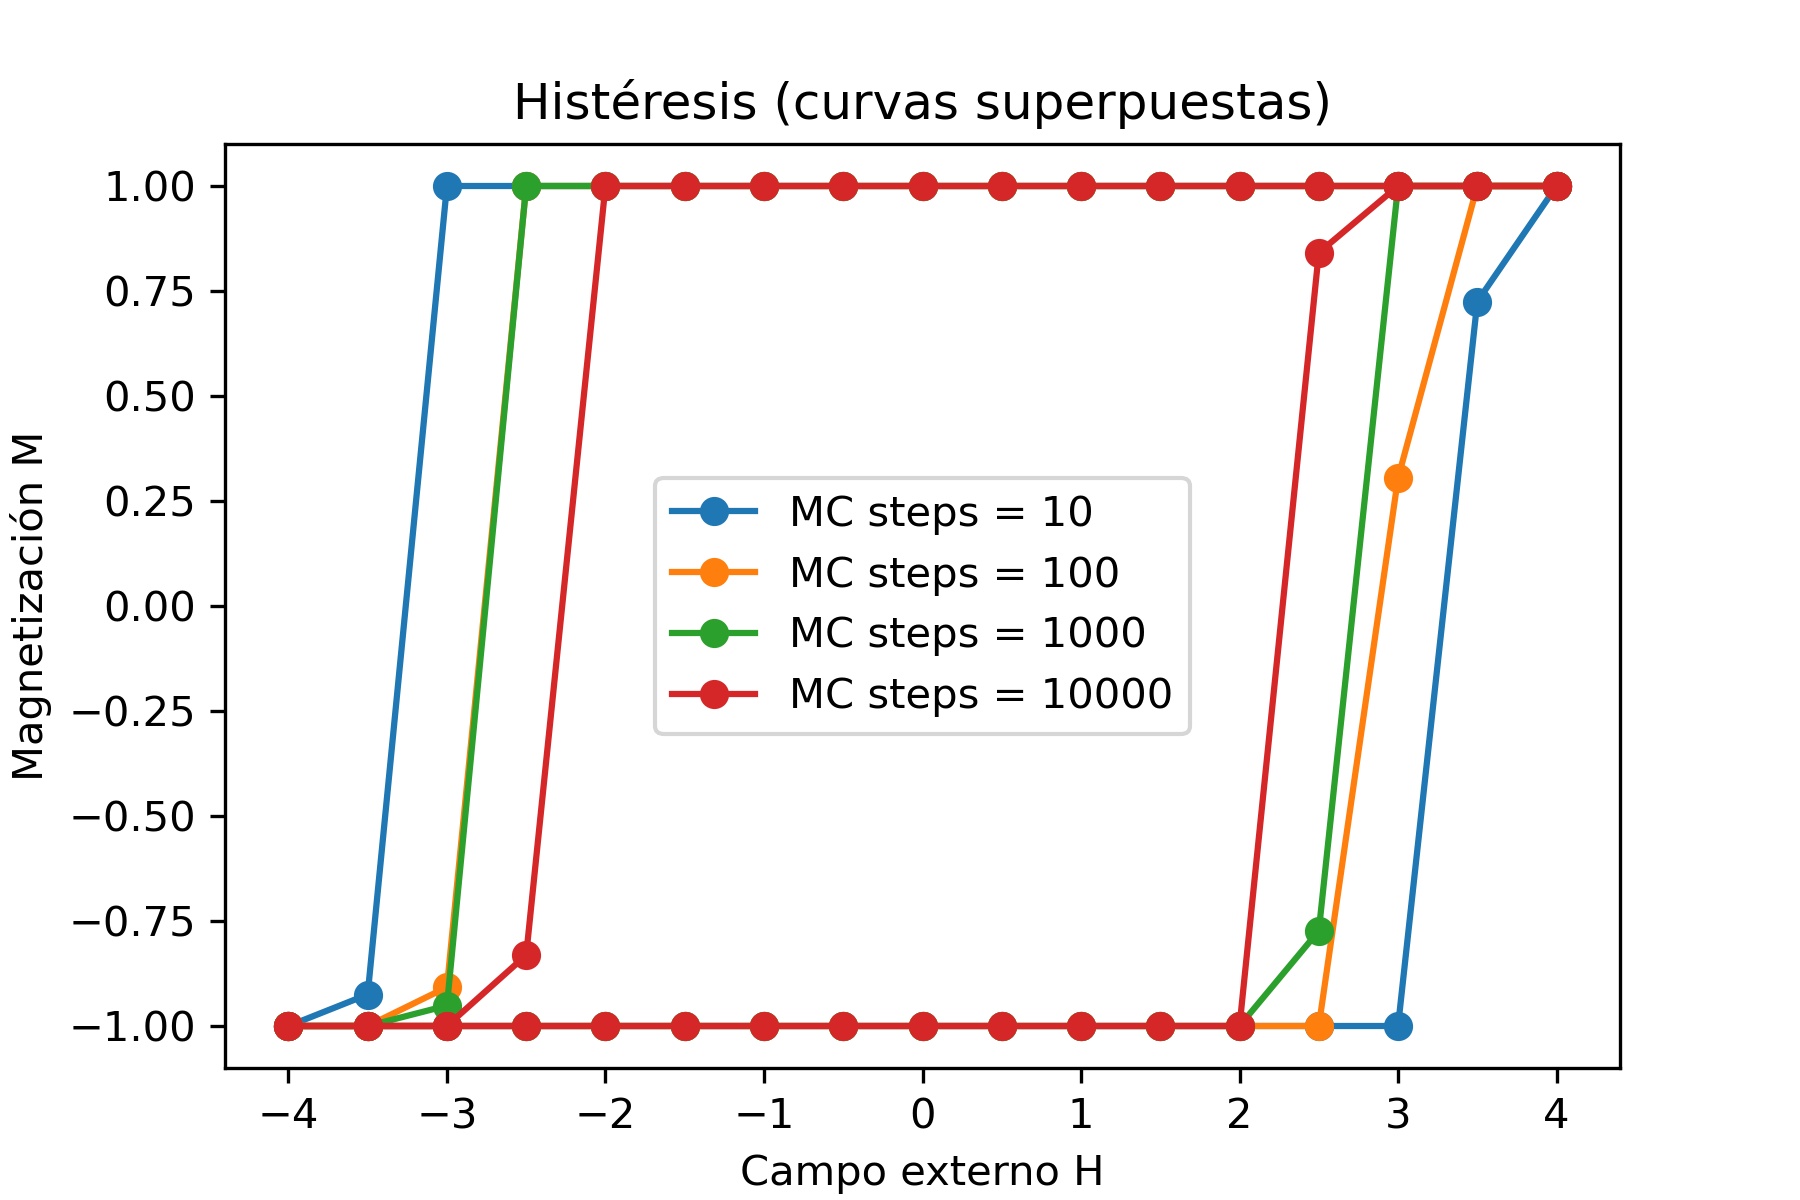
\includegraphics[width=0.5\textwidth]{imagenes/histeresis_global.png}
\caption{Curvas de histéresis de la magnetización para distintos tiempos de Monte Carlo cuando $T=0.25$.}
\label{fig:histeresis_global}
\end{figure}

\begin{figure}[H]
\centering
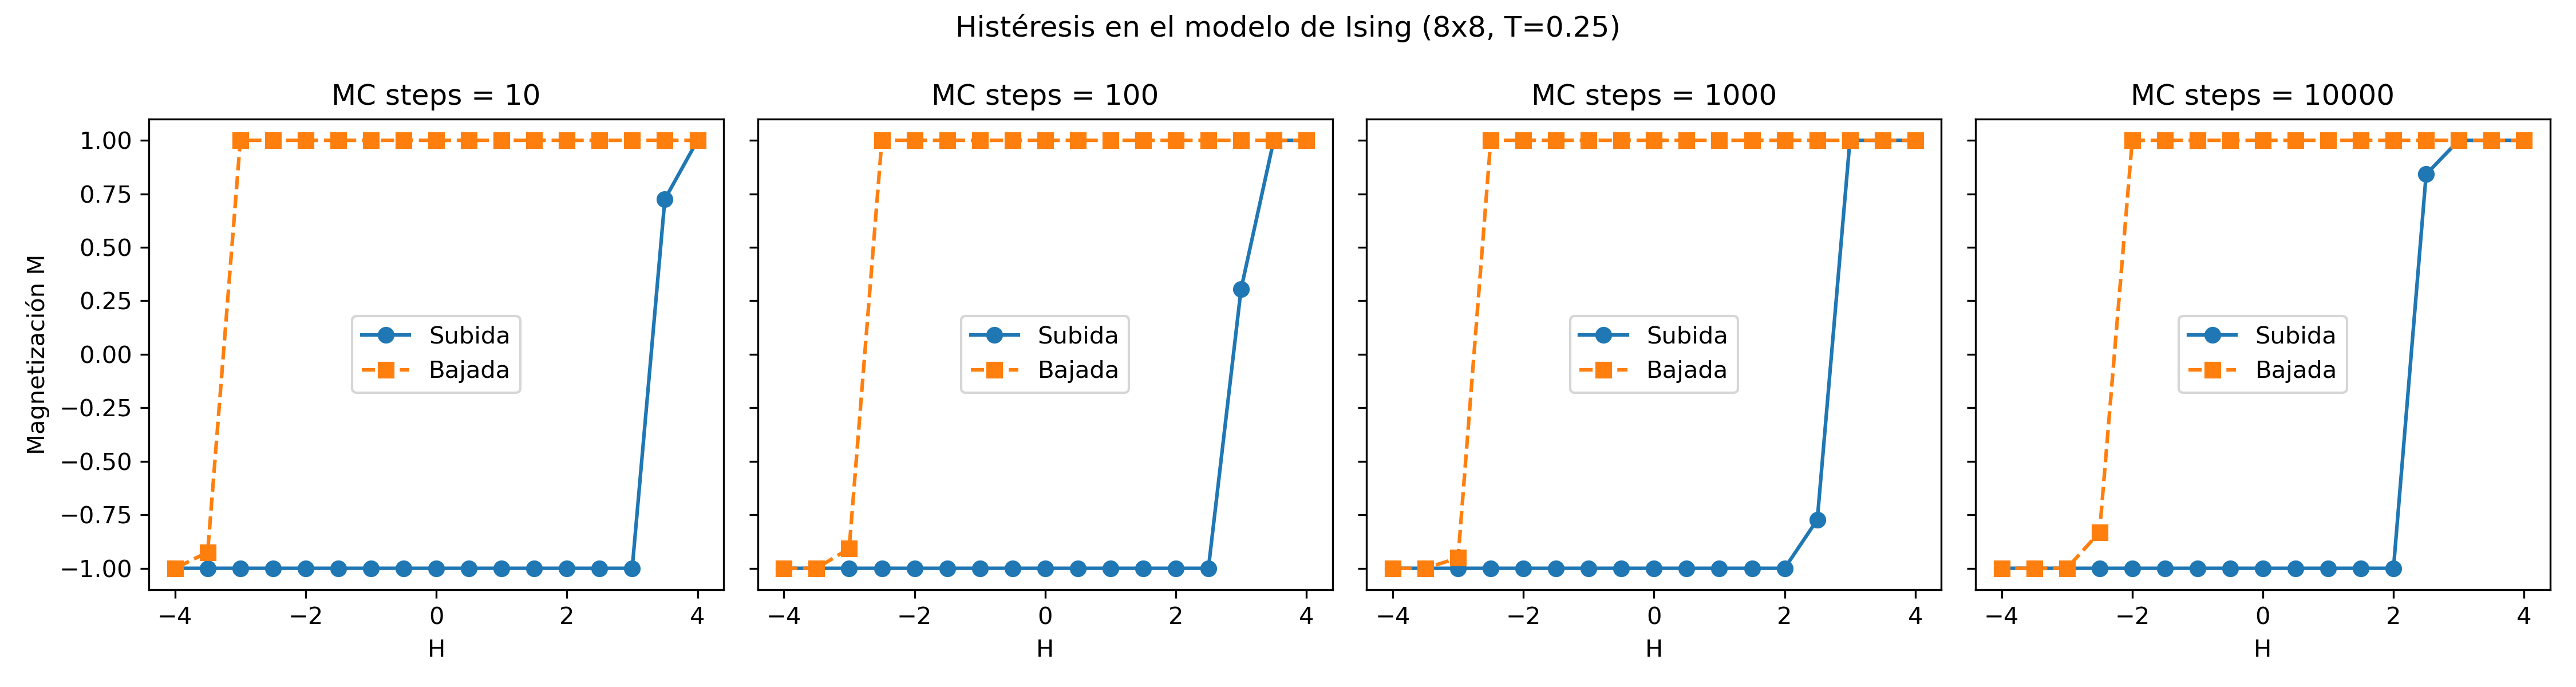
\includegraphics[width=\textwidth]{imagenes/histeresis_subplots.png}
\caption{Curvas de histéresis para distintos números de pasos de Monte Carlo.}
\label{fig:histeresis_subplots}
\end{figure}

Se observa claramente que para un número pequeño de pasos de Monte Carlo, el sistema presenta un bucle de histéresis amplio. A medida que aumenta el número de pasos, el área del bucle disminuye, lo que significa que se acerca progresivamente al equilibrio termodinámico aunque el sistema sigue sin tener tiempo suficiente para reorganizar sus espines ante variaciones rápidas del campo magnético.

\subsection{Dependencia con la temperatura}

En las Figura~\ref{fig:magnetizacion_hist} se muestran los ciclos de histéresis de la magnetización en función del campo magnético externo para diferentes temperaturas.

\begin{figure}[H]
\centering
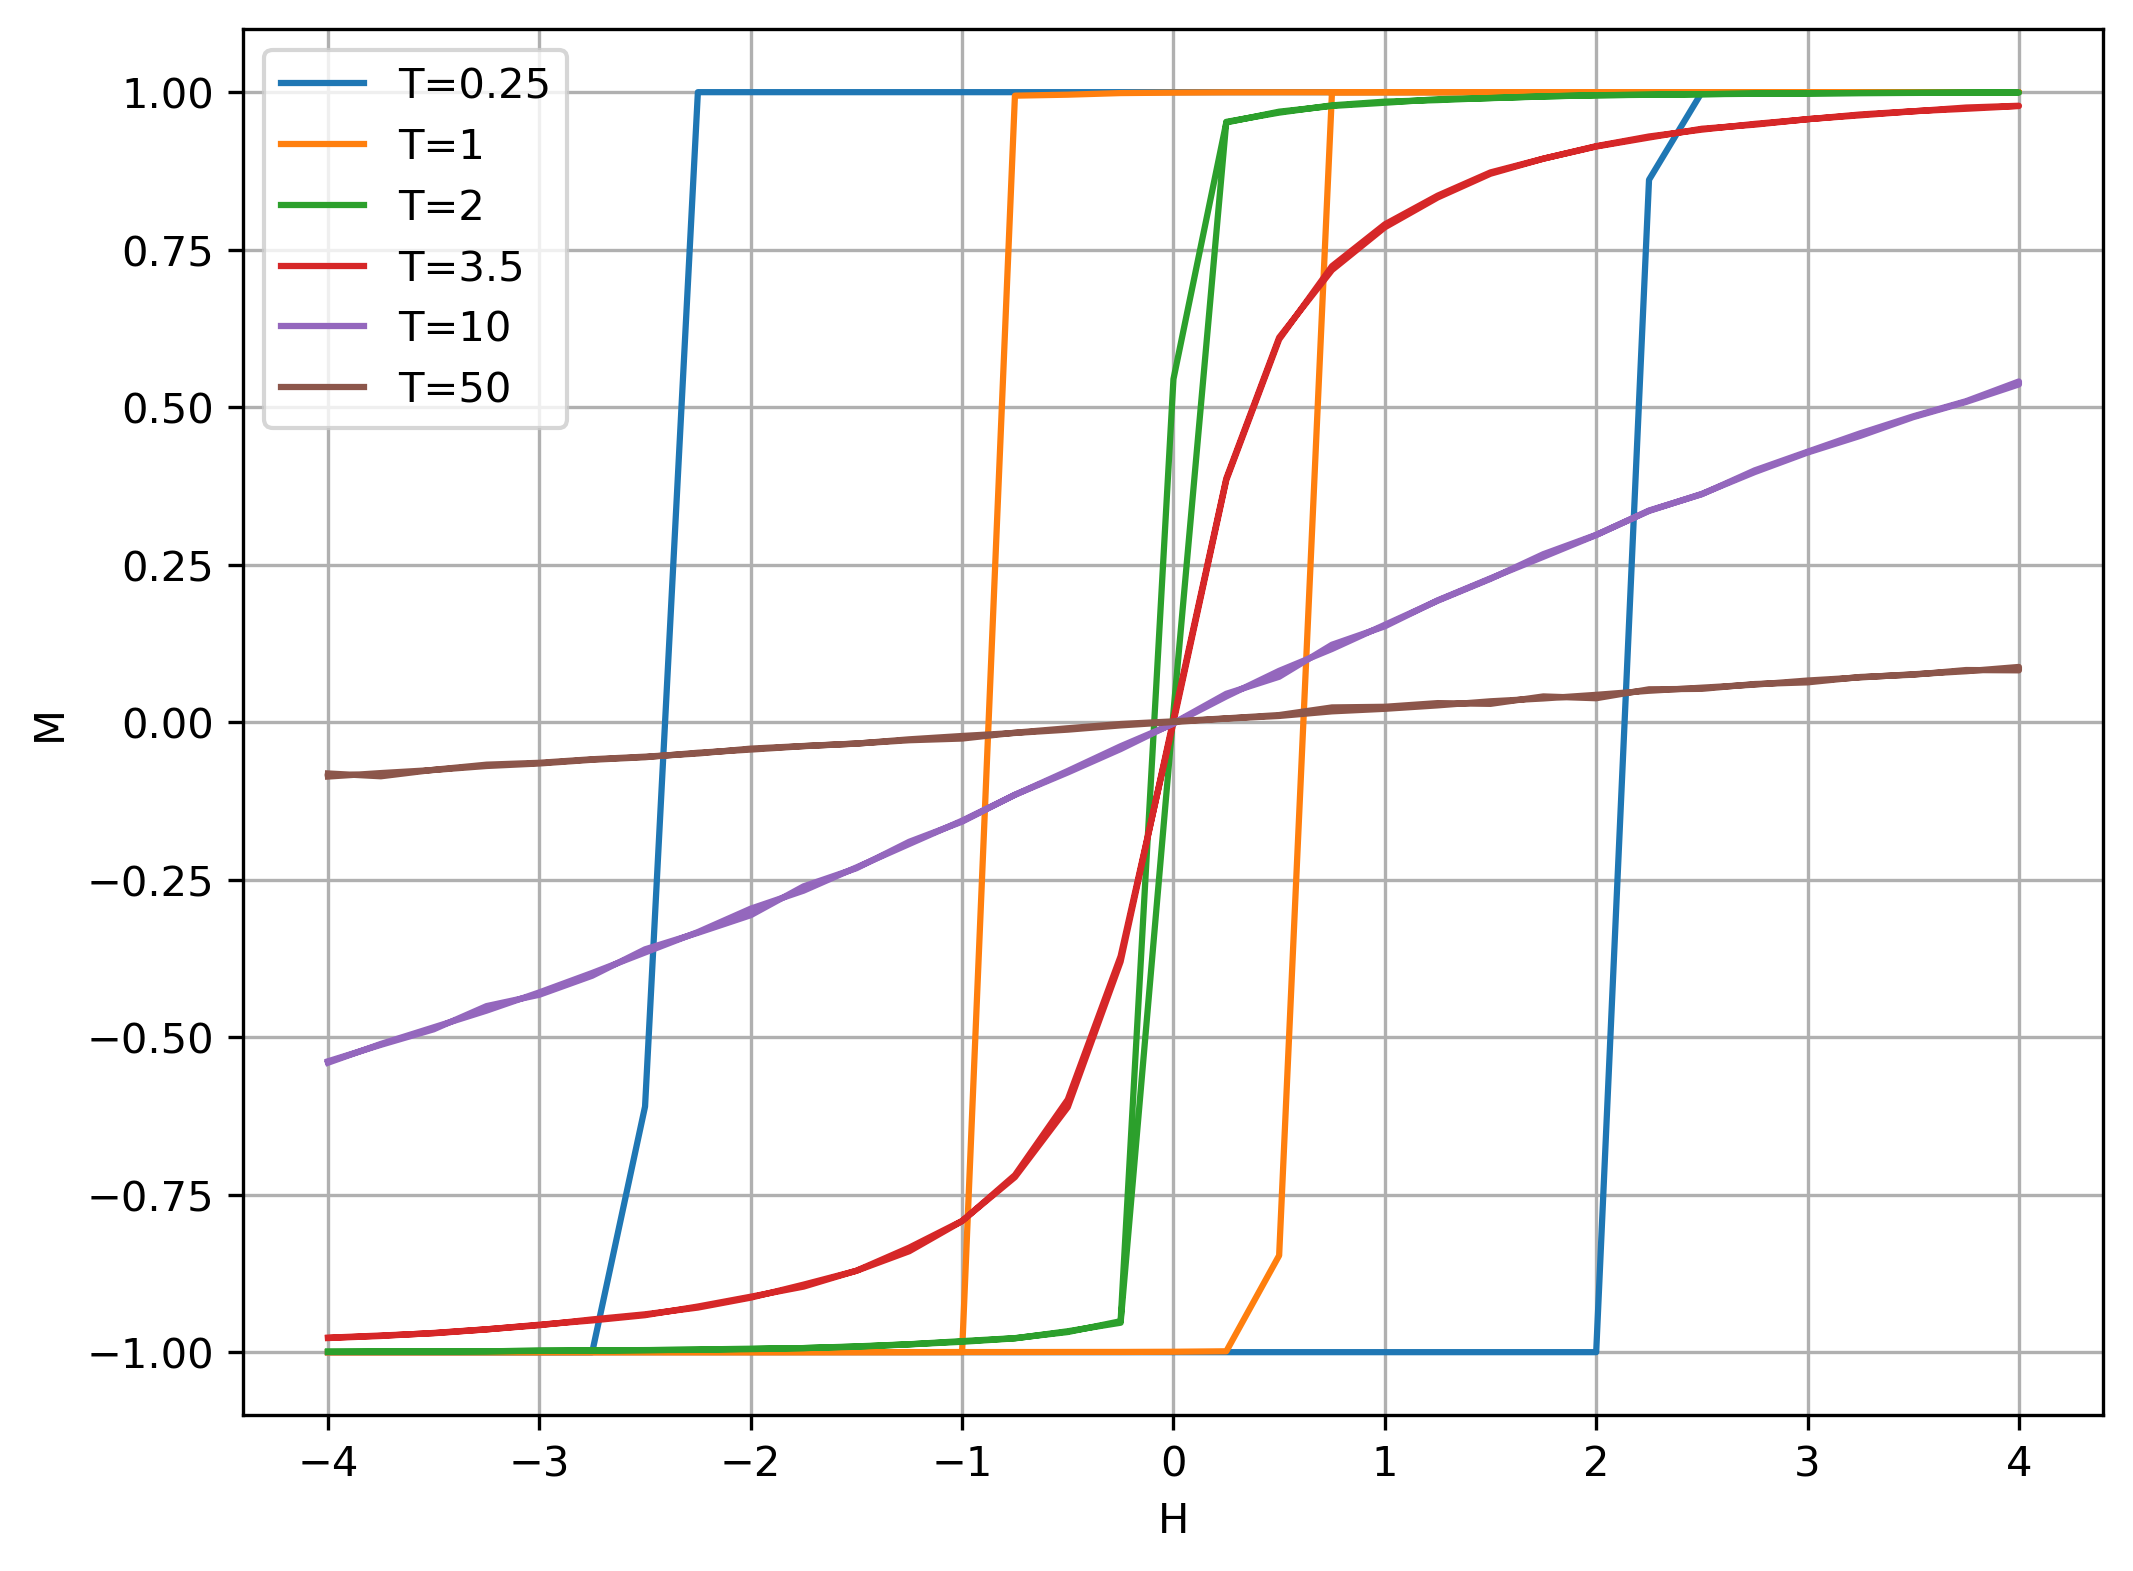
\includegraphics[width=0.5\textwidth]{imagenes/magnetizacion_hist_final.png}
\caption{Magnetización en función del campo externo para diferentes temperaturas.}
\label{fig:magnetizacion_hist}
\end{figure}

\begin{figure}[H]
\centering
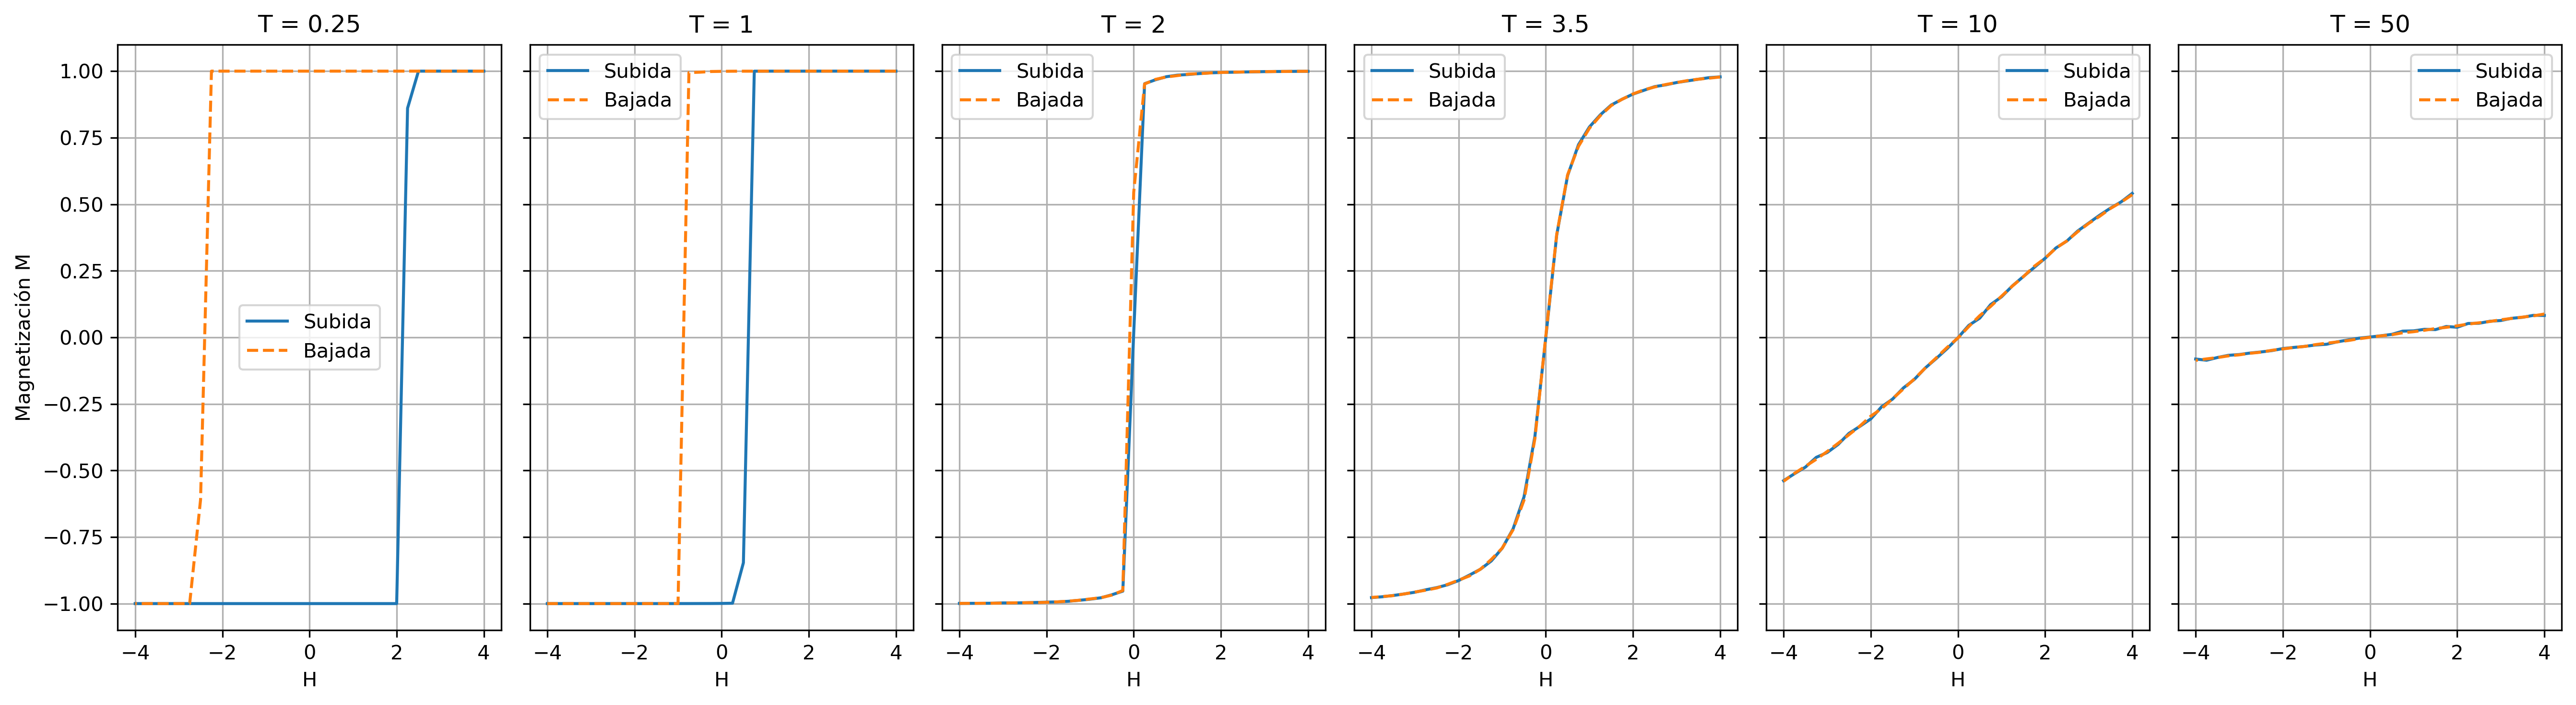
\includegraphics[width=\textwidth]{imagenes/histeresis_vs_temperatura_subplots.png}
\caption{Evolución de ciclos de histéresis de la magnetización para distintas temperaturas.}
\label{fig:histeresis_vs_temperatura}
\end{figure}

Los resultados muestran que a bajas temperaturas ($T = 0.25$), el sistema presenta un bucle de histéresis pronunciado. A medida que aumenta la temperatura, el tamaño del ciclo de histéresis se reduce hasta que a temperaturas altas prácticamente desaparece. Además, si la temperatura es suficientemente alta, el sistema no se llega a encontrar nunca completamente ordenado en el rango de valores estudiados del campo magnético. Este comportamiento se debe al aumento de la temperatura, que permite al sistema alcanzar el equilibrio más rápidamente y reduce la importancia de las barreras energéticas del sistema.

\subsection{Energía en función del campo externo}

En la Figura \ref{fig:energia_hist} se representa la energía media del sistema en función del campo externo, diferenciando entre el barrido ascendente y descendente, para diferentes temperaturas.

\begin{figure}[H]
\centering
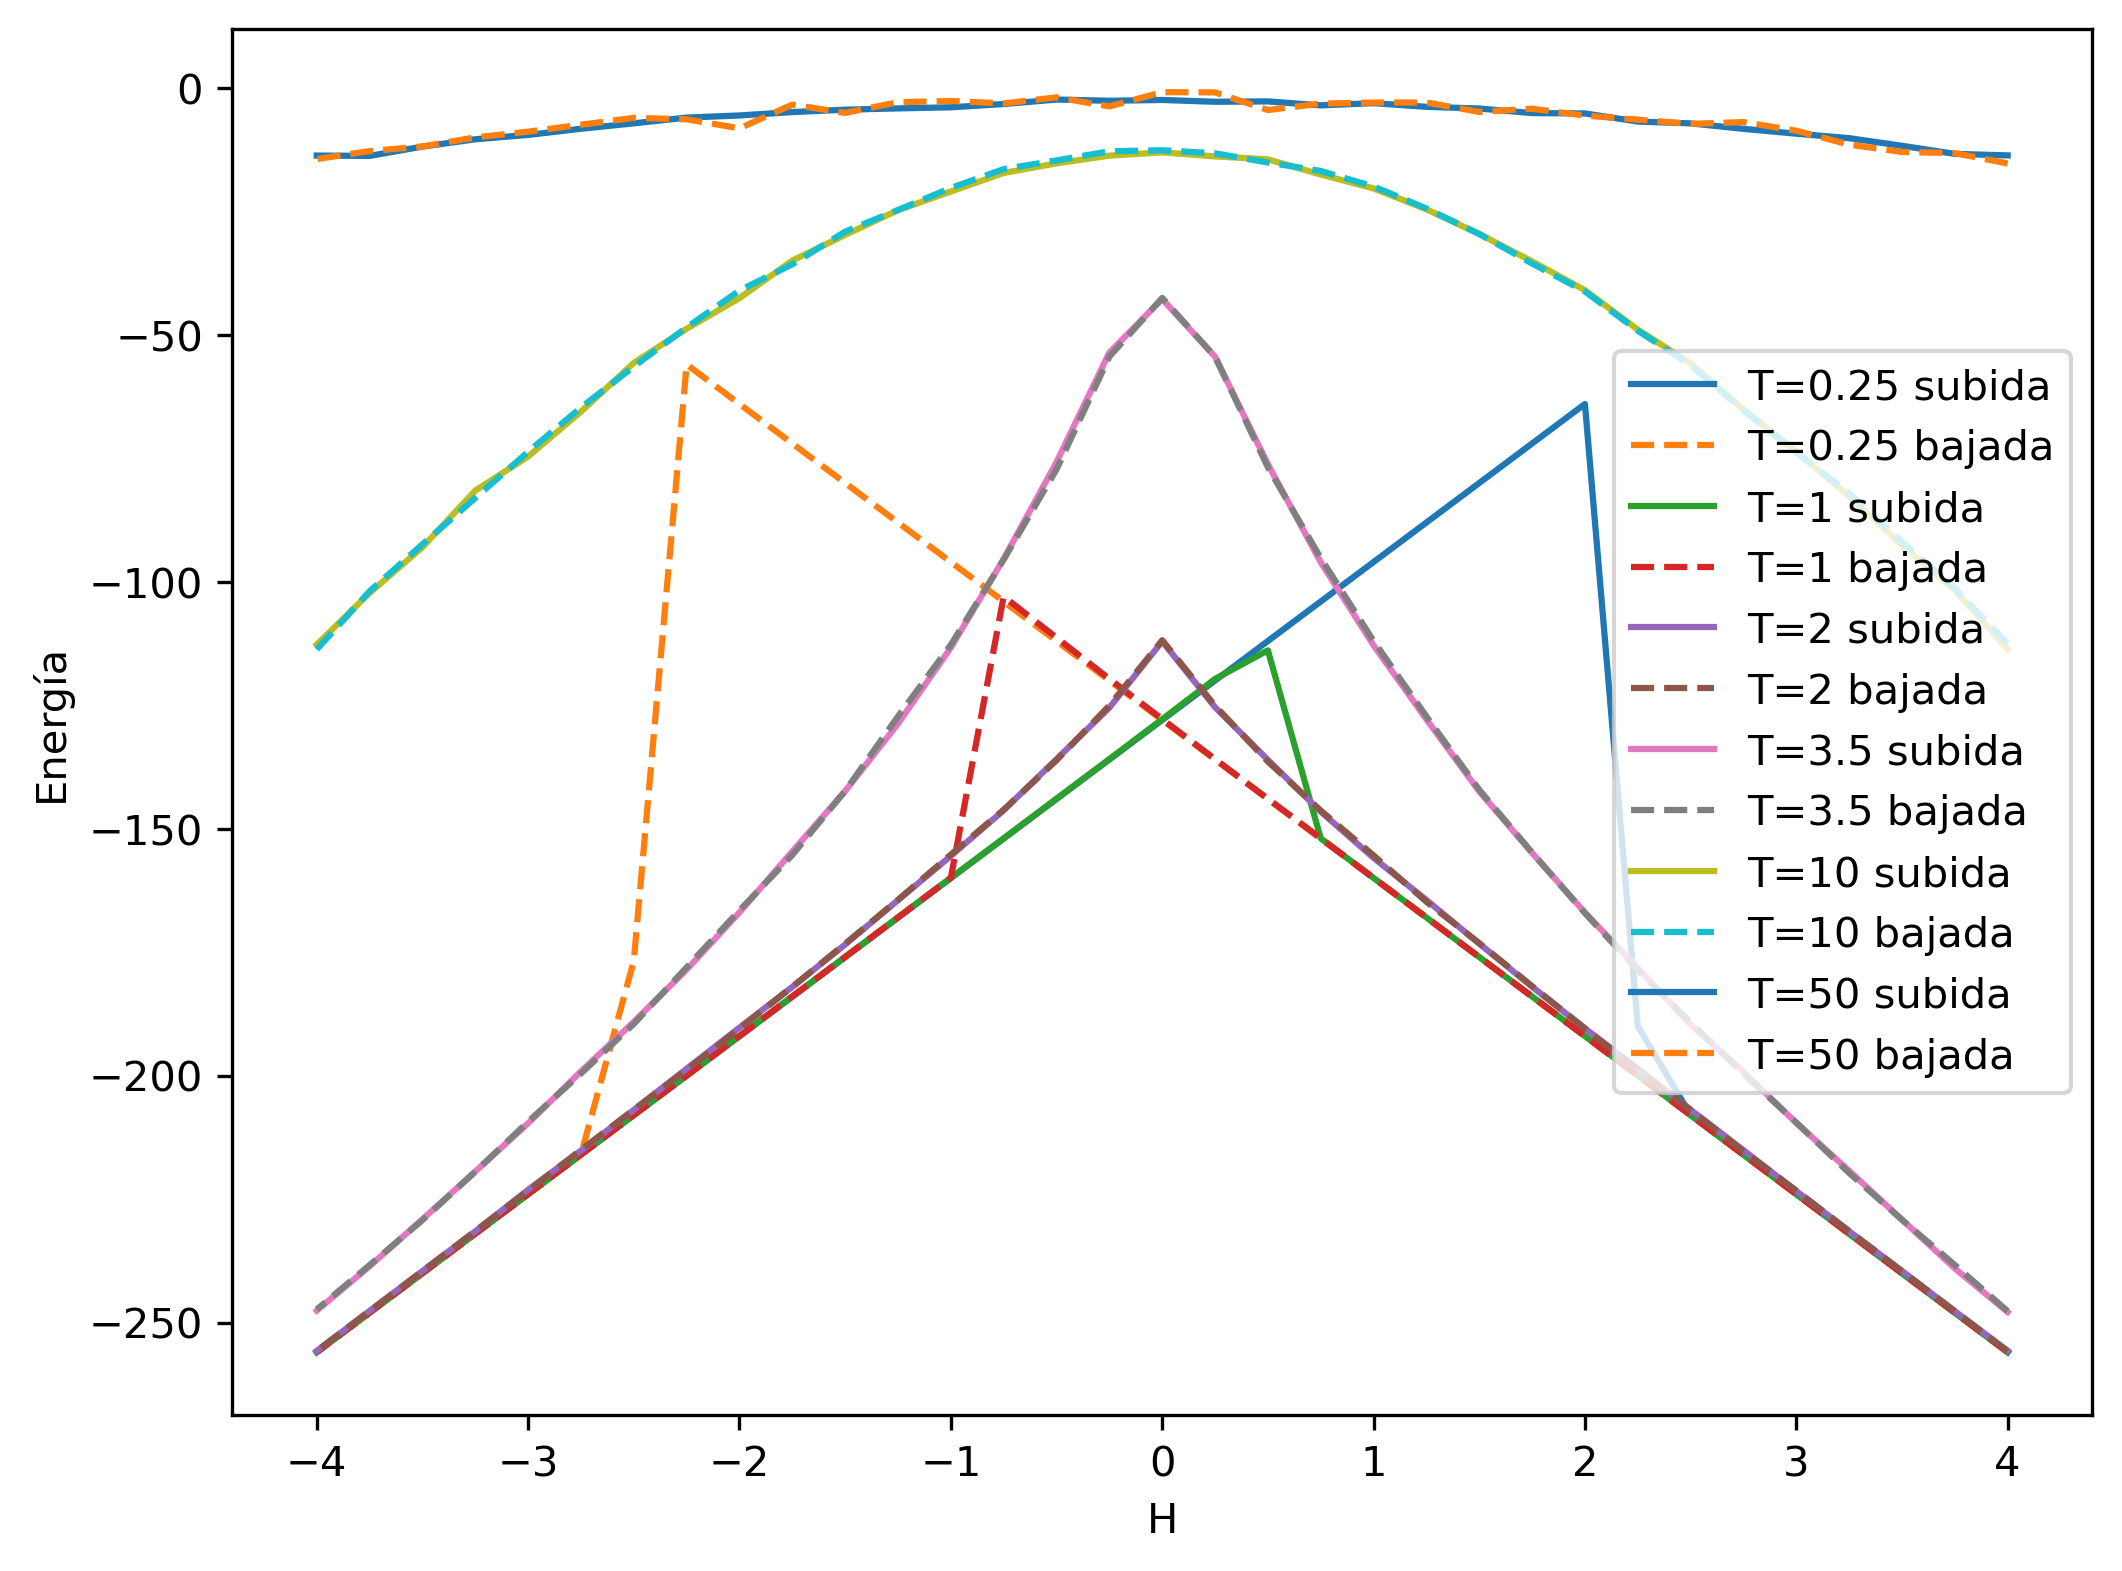
\includegraphics[width=0.7\textwidth]{imagenes/energia_hist_final.png}
\caption{Energía en función del campo externo para diferentes temperaturas.}
\label{fig:energia_hist}
\end{figure}

\begin{figure}[H]
\centering
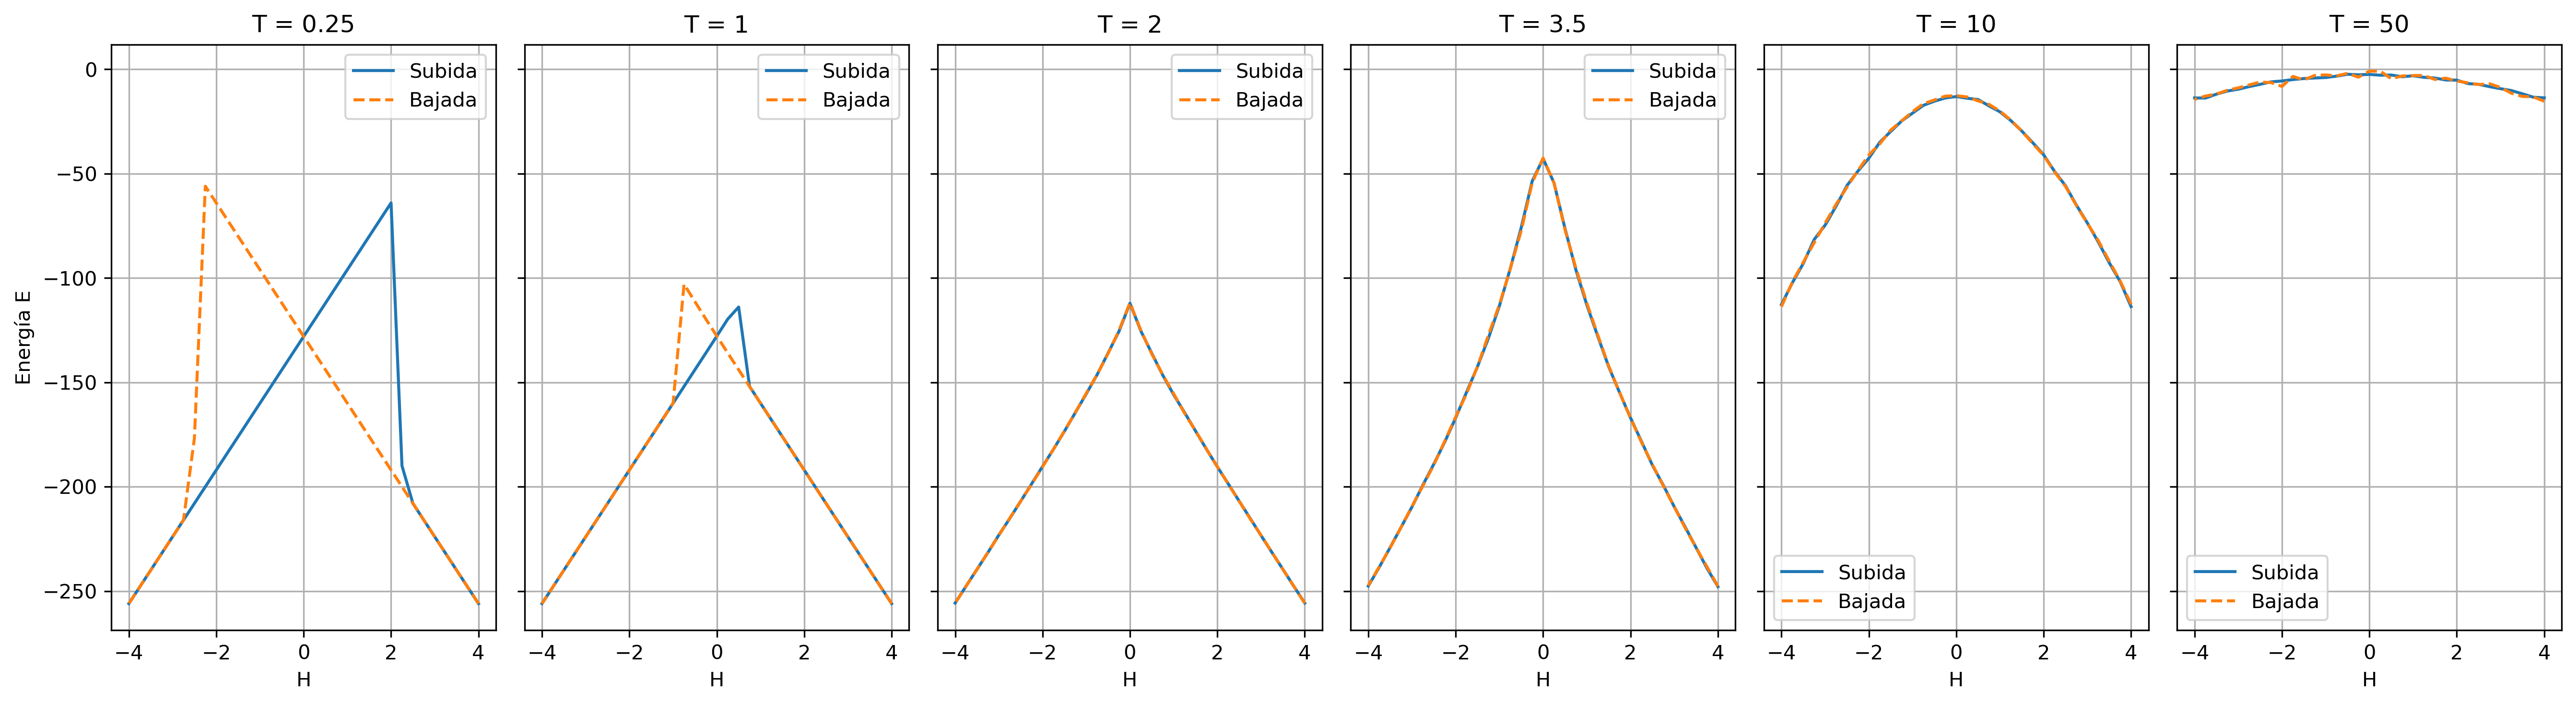
\includegraphics[width=\textwidth]{imagenes/energia_vs_temperatura_subplots.png}
\caption{Energía en función del campo para distintas temperaturas en gráficas individuales.}
\label{fig:energia_subplots}
\end{figure}

Se observa que la energía presenta un comportamiento distinto en la subida y bajada del campo. Como ocurre con la magnetización, este efecto es más notable a bajas temperaturas, mientras que a altas temperaturas, ambas curvas tienden a coincidir.

Este resultado indica la presencia de histéresis también en la energía. Como la energía depende de la magnetización, la histéresis se manifiesta también en la energía cuando el sistema se encuentra fuera del equilibrio.

\subsection{Energía en función de la temperatura para campo fijo}

En la Figura~\ref{fig:energia_vs_T_global} se representa la energía media del sistema en función de la temperatura para varios valores de $H$, obteniendo otra perspectiva para analizar el comportamiento de E(T,H)

\begin{figure}[H]
\centering
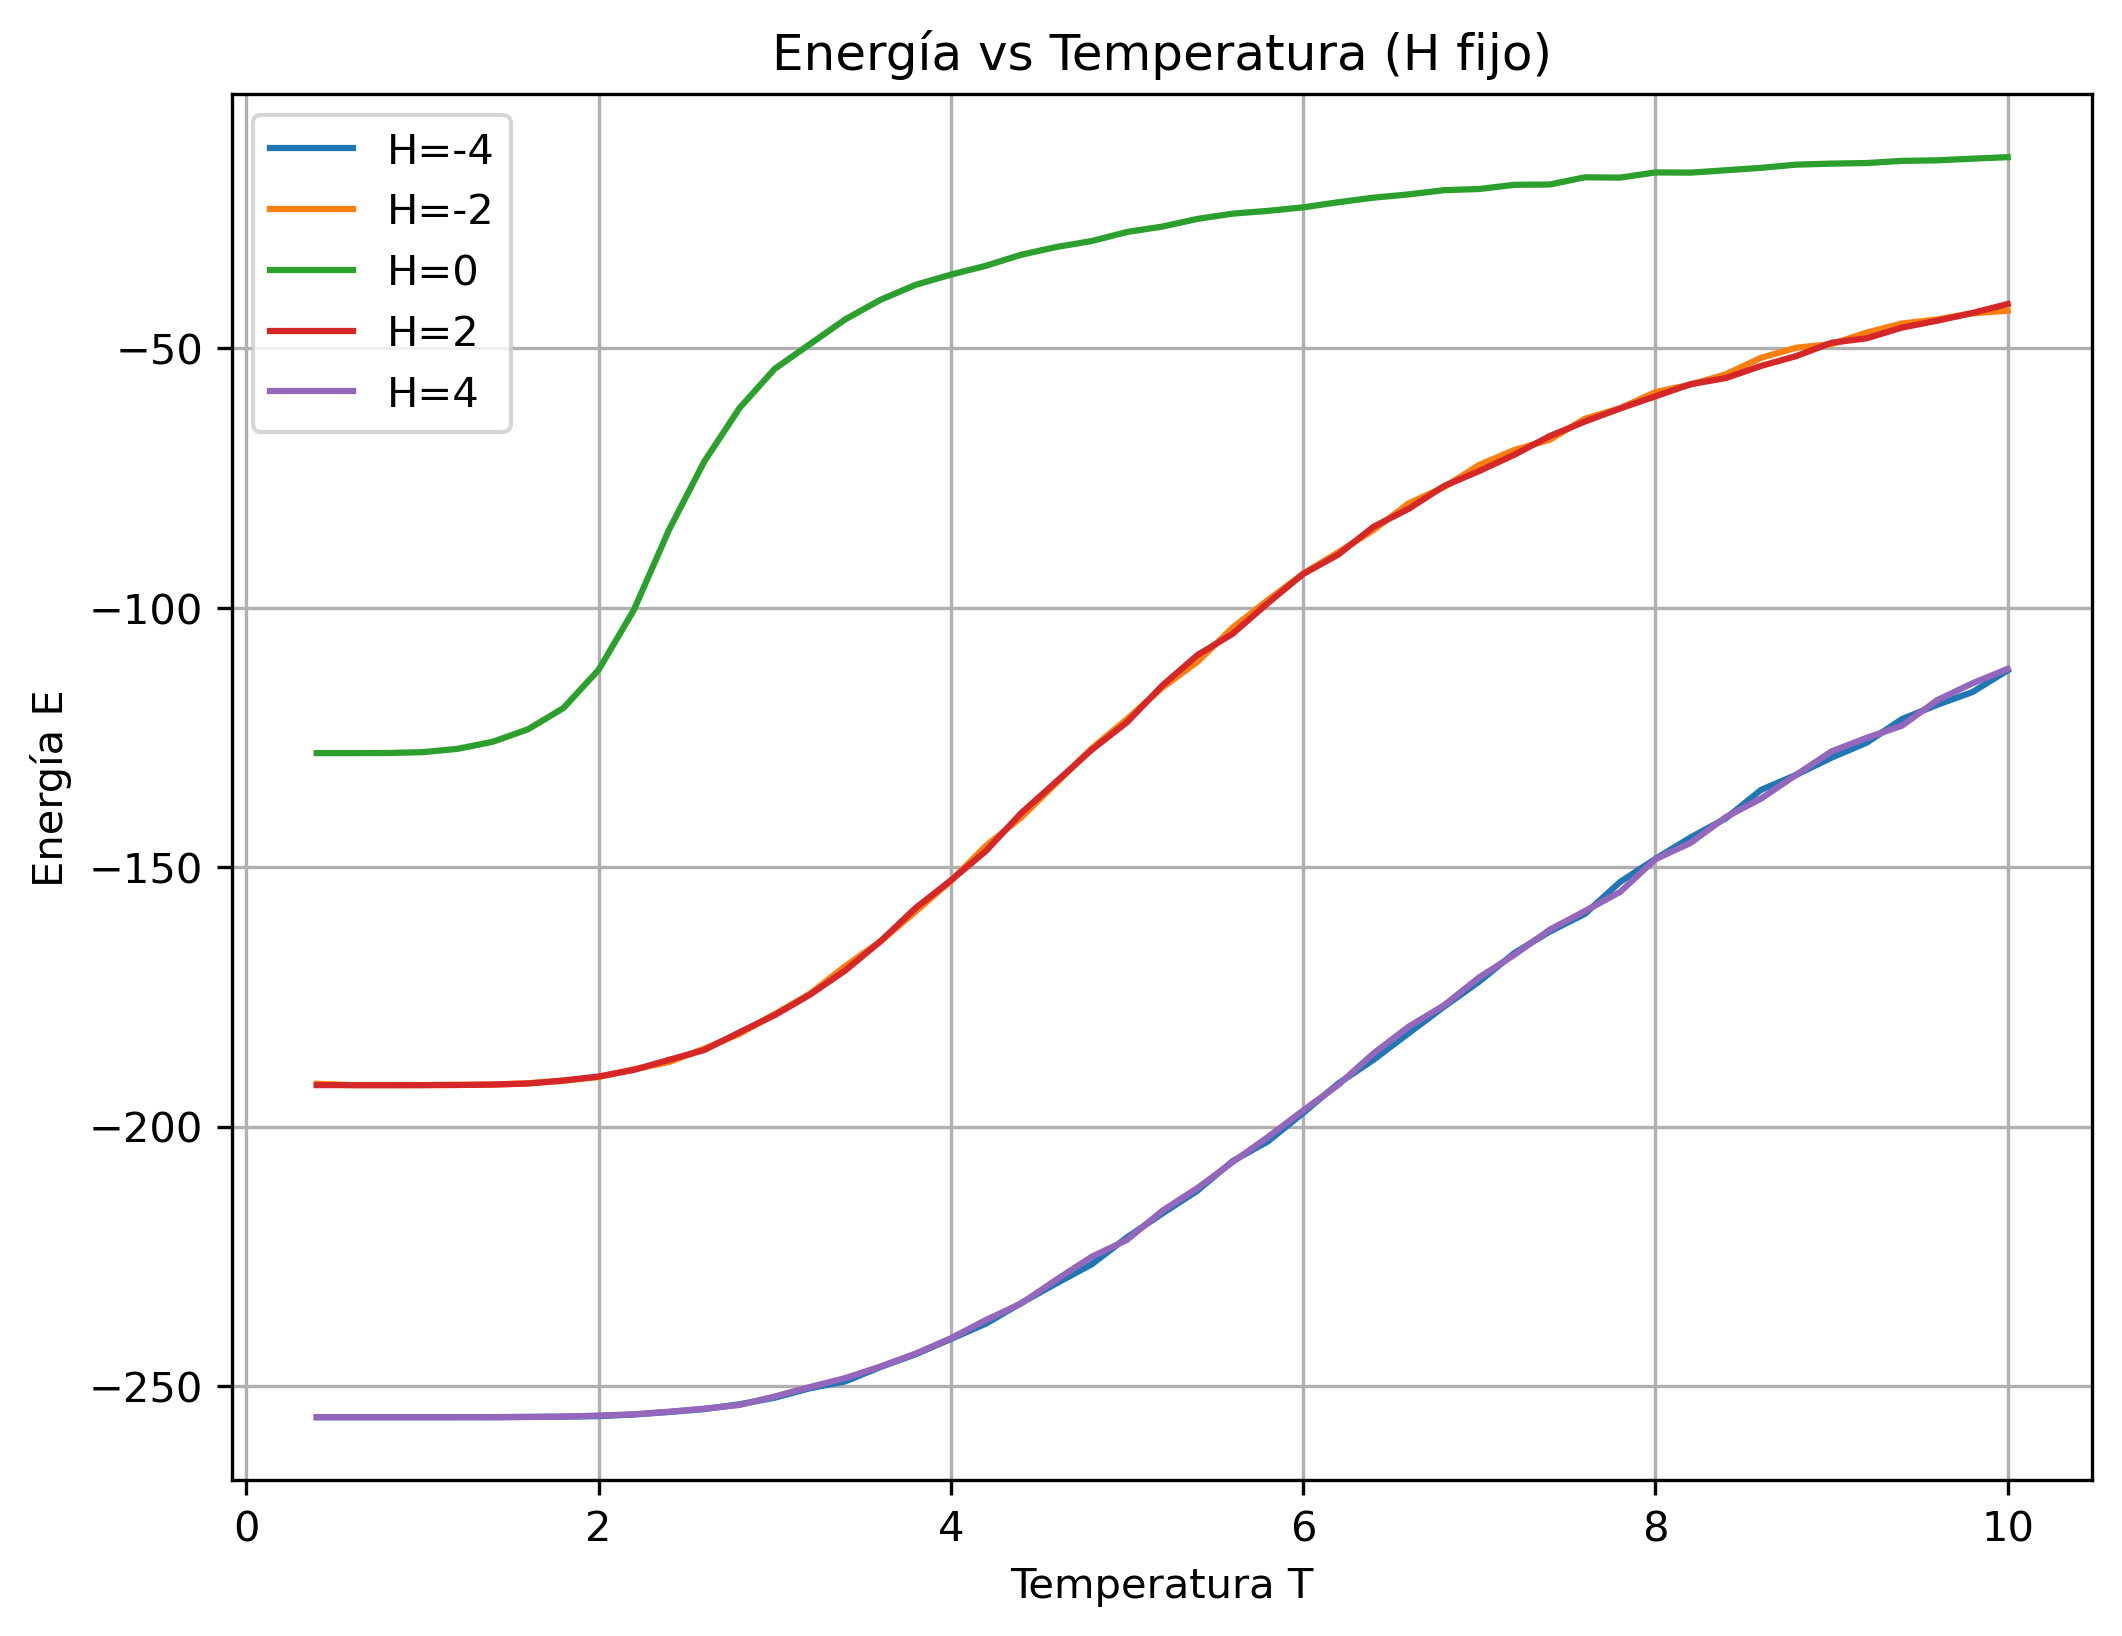
\includegraphics[width=0.7\textwidth]{imagenes/energia_vs_T_global_zoom.png}
\caption{Energía en función de la temperatura para distintos valores del campo magnético externo.}
\label{fig:energia_vs_T_global}
\end{figure}

Adicionalmente, en la Figura~\ref{fig:energia_vs_T_subplots} se muestran estas mismas curvas en gráficos individuales para cada valor de $H$, por claridad.

\begin{figure}[H]
\centering
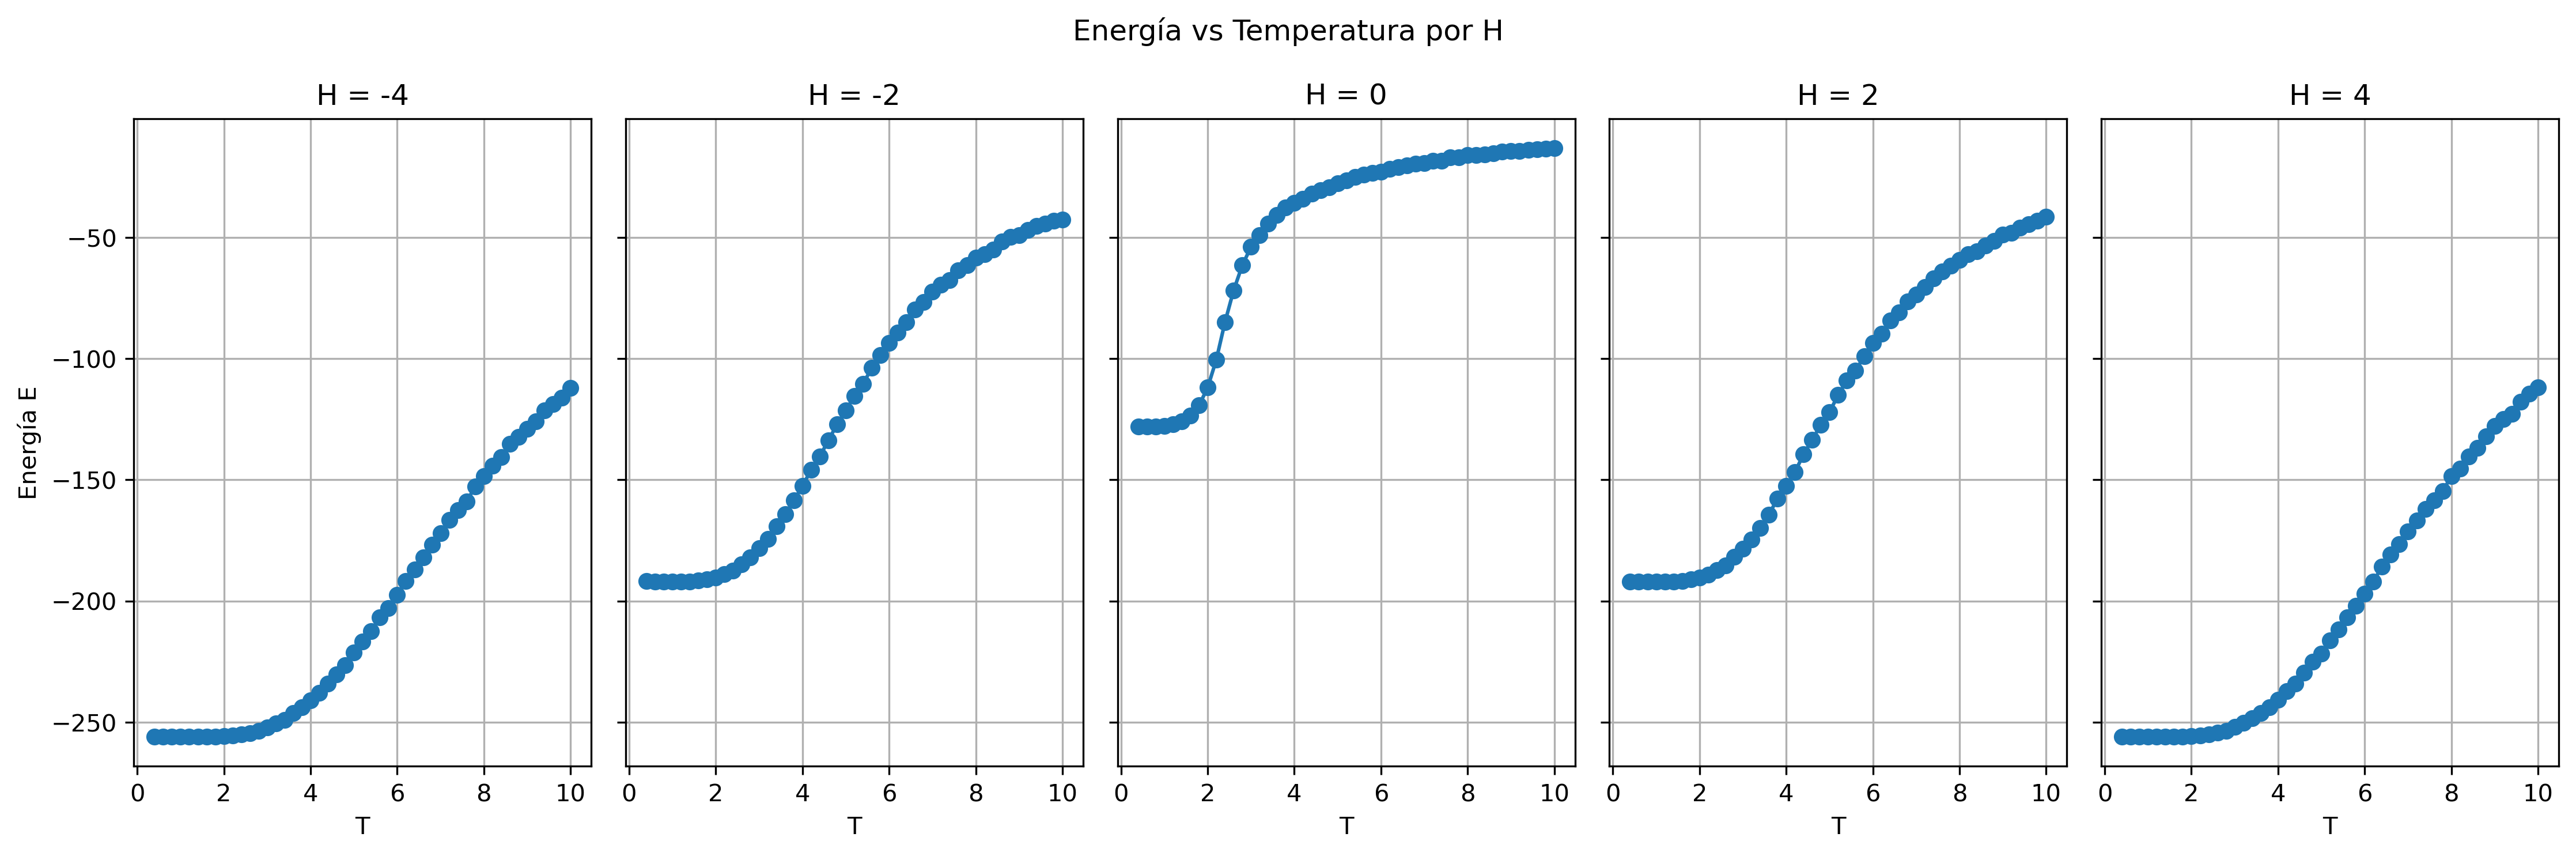
\includegraphics[width=\textwidth]{imagenes/energia_vs_T_subplots_zoom.png}
\caption{Energía en función de la temperatura para distintos valores de $H$ en gráficos individuales.}
\label{fig:energia_vs_T_subplots}
\end{figure}

En primer lugar, al aumentar el valor absoluto del campo magnético externo, se observa que la energía del sistema toma valores más bajos en todo el rango de temperaturas. Este comportamiento se debe al término $-H \sum_i s_i$ del Hamiltoniano del sistema, que favorece configuraciones alineadas con el campo y reduce la energía total.

Por otro lado, se sigue observando que la energía aumenta con la temperatura para todos los valores del campo magnético. Este comportamiento es consistente con el hecho de que al incrementar $T$ aumentan las fluctuaciones, lo que favorece configuraciones más desordenadas, es decir, con energías más cercanas a 0. Además se observa que la transición hacia los estados desordenados (de energía cercana a 0) es más lenta para valores mayores de $|H|$, ya que el campo favorece la alineación de los espines en una dirección preferente, lo que estabiliza configuraciones de menor energía incluso a temperaturas relativamente altas.

En conjunto, estos resultados exponen que tanto la temperatura como el campo magnético externo controlan el grado de orden y la energía del sistema.

\section{Conclusiones}

Los resultados obtenidos muestran claramente que la histéresis disminuye al aumentar el número de pasos Monte Carlo, debido a la mejor relajación del sistema; además, la histéresis desaparece al aumentar la temperatura por encima de la temperatura crítica. 

Así, existe una transición de fase entre un régimen ordenado (bajas temperaturas) y un régimen desordenado (altas temperaturas). Por otro lado, el sistema presenta memoria a bajas temperaturas, lo cual es característico del estado ferromagnético.

Finalmente, el estudio de $E(H,T)$ exponer que tanto la temperatura como el campo magnético externo controlan el grado de orden y la energía total del sistema. Como regla general, se observa que el aumento de T aumenta la energía del sistema mientras que el aumento de $|H|$ provoca que la energía del sistema disminuya y que el sistema se oponga a cambios bruscos de ordenamiento debido a la temperatura.

\begin{thebibliography}{9}

\bibitem{giordano}
N. J. Giordano and H. Nakanishi,
\textit{Computational Physics},
2nd ed., Pearson Prentice Hall, 2006.
\label{Giordano}
\end{thebibliography}

\appendix
\section*{Anexo A: Variables y parámetros del modelo}

\begin{center}
\begin{tabular}{ll}
\hline
\textbf{Variable} & \textbf{Significado} \\
\hline
$s_i$ & Espín en el sitio $i$, toma valores $\pm 1$ \\
$N$ & Tamaño lineal de la red ($N \times N$) \\
$J$ & Constante de acoplamiento ferromagnético \\
$H$ & Campo magnético externo \\
$E$ & Energía total del sistema \\
$M$ & Magnetización media por espín \\
$T$ & Temperatura del sistema \\
$k_B$ & Constante de Boltzmann (tomada como 1) \\
$\Delta E$ & Variación de energía al intentar invertir un espín \\
$\langle i,j \rangle$ & Suma sobre pares de primeros vecinos \\
$nn$ & Conjunto de vecinos más próximos \\
\\
$n_{eq}$ & Número de pasos de equilibración entre medidas \\
$n_{meas}$ & Número de medidas para promediar magnitudes \\
$mc\_steps$ & Número de pasos Monte Carlo por valor de $H$ \\
\\
$H_{max}$ & Valor máximo del campo magnético en el barrido \\
$\Delta H$ & Incremento del campo magnético \\
$H_{up}$ & Barrido ascendente del campo magnético \\
$H_{down}$ & Barrido descendente del campo magnético \\
\\
$T_{values}$ & Conjunto de temperaturas estudiadas \\
$H_{fijos}$ & Valores fijos de campo para estudiar $E(T)$ \\
\\
$\exp(-\Delta E / k_B T)$ & Probabilidad de aceptación de Metropolis \\
\\
$M(H)$ & Magnetización en función del campo magnético \\
$E(H)$ & Energía en función del campo magnético \\
$E(T)$ & Energía en función de la temperatura \\
\\
$T_c$ & Temperatura crítica del modelo de Ising 2D ($\approx 2.26$) \\
\hline
\end{tabular}
\end{center}

\section*{Anexo B: Gráficas completas de la evolución de la energía con la temperatura}

Adicionalmente, en las Figuras ~\ref{ll} y~\ref{fig:energia_vs_T_subplots_total} se muestran las gráficas E(T) para diferentes valores de H hasta una temperatura mayor que en las figuras del informe para observar que, finalmente, el aumento de temperatura lleva al desorden total del sistema.

\begin{figure}[H]
\centering
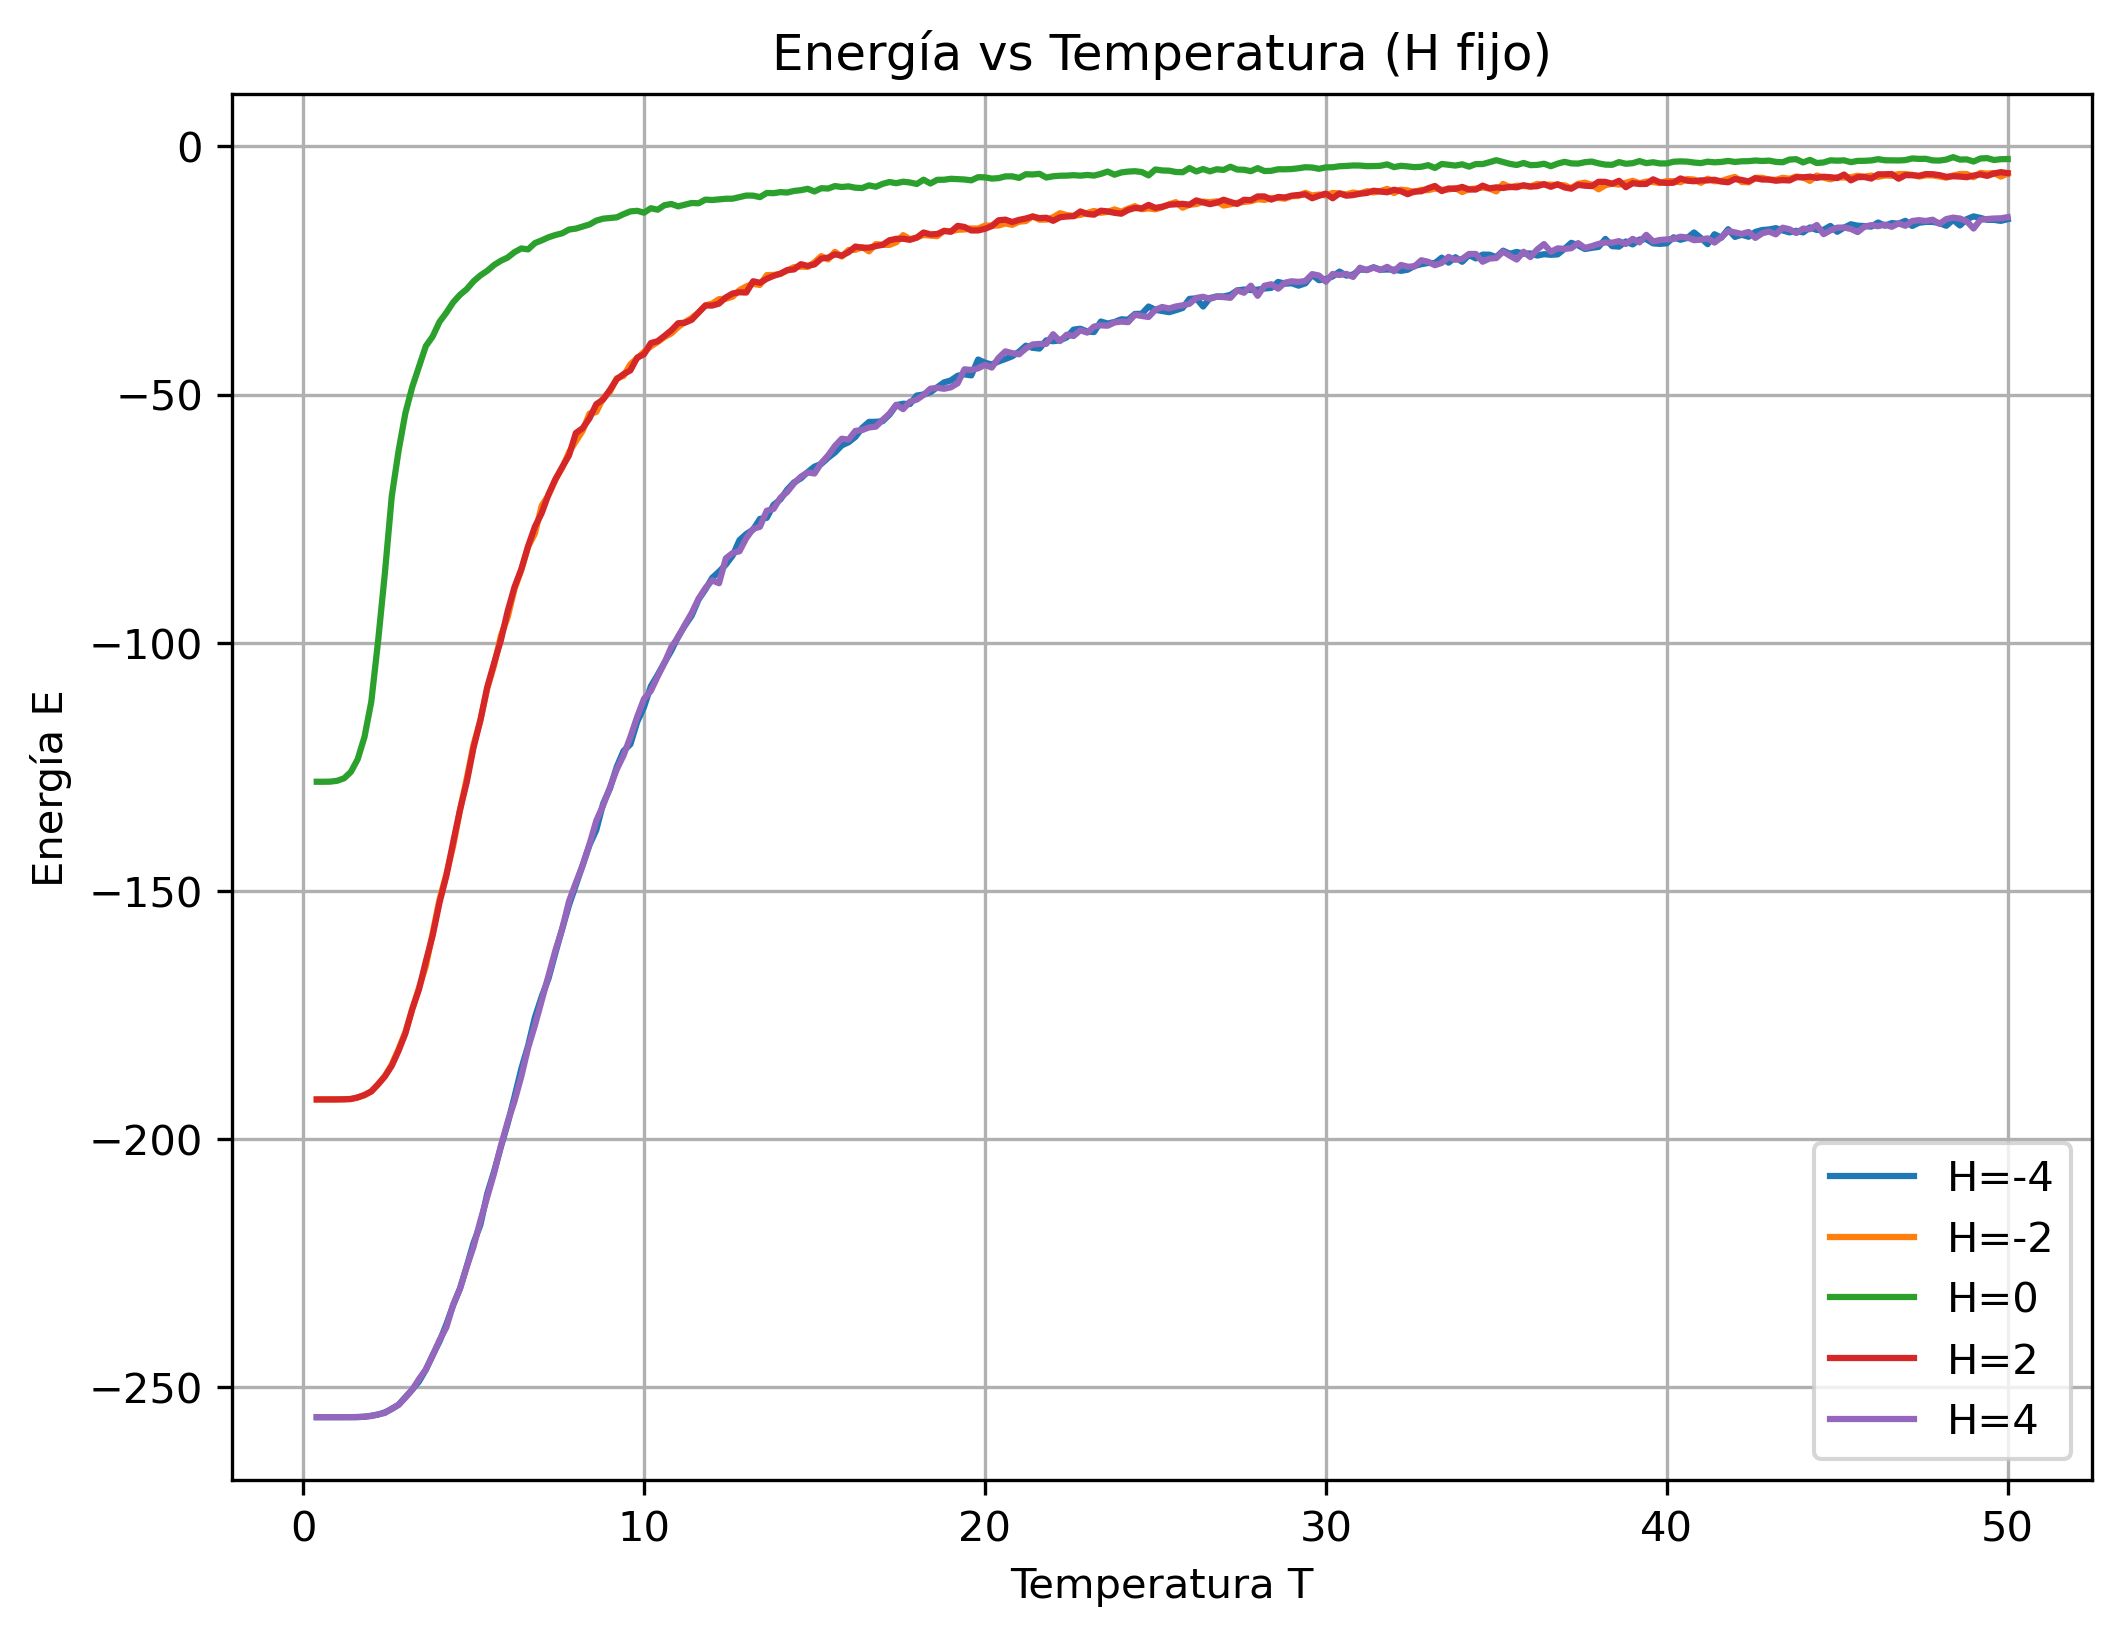
\includegraphics[width=0.7\textwidth]{imagenes/energia_vs_T_global.png}
\caption{Energía en función de la temperatura para distintos valores del campo magnético externo.}
\label{ll}
\end{figure}

\begin{figure}[H]
\centering
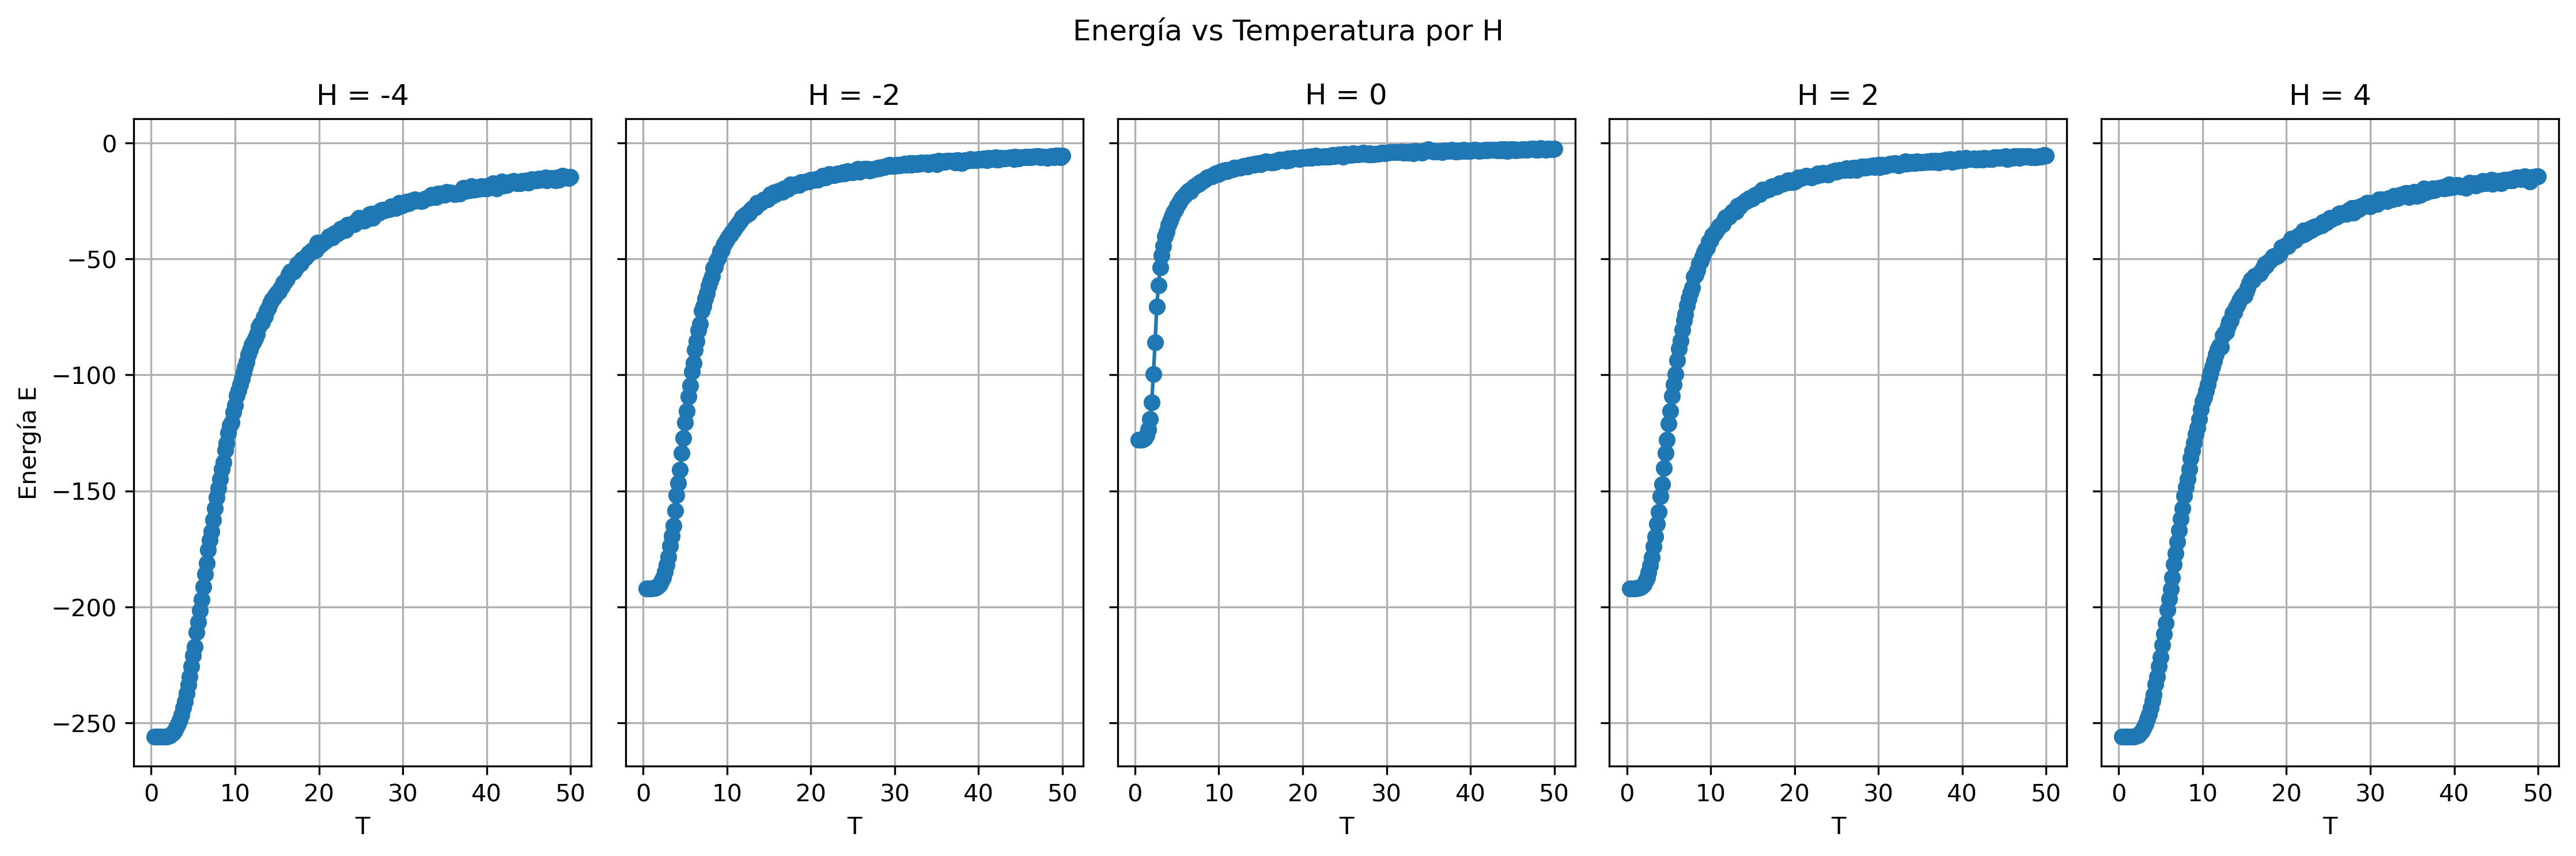
\includegraphics[width=\textwidth]{imagenes/energia_vs_T_subplots.png}
\caption{Energía en función de la temperatura para distintos valores de $H$ en gráficos individuales.}
\label{fig:energia_vs_T_subplots_total}
\end{figure}

\end{document}